\section{Příklad 1}
% Jako parametr zadejte skupinu (A-H)
\prvniZadani{A}

\large{\textbf{Řešení:}}

%%% Krok 1 - Zjednodušení paralelných rezistorů
\begin{center}
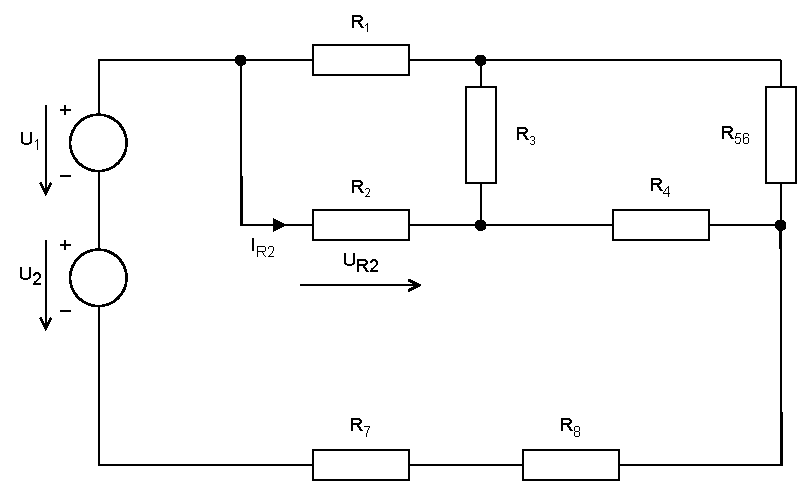
\includegraphics[scale=0.8,keepaspectratio]{fig/solutions/01-sol/01-step1.pdf} \\
Obr.1.1 - Zjednodušení paralelných rezistorů
($R_5, R_6 \Rightarrow R_{56}$)
\end{center}

\begin{gather*}
R_{56} = \frac{R_5 \times R_6}{R_5 + R_6} = \frac{360 \times 750}{360 + 750} = 243.24324324 \Omega
\end{gather*}

\newpage

%%% Krok 2 - Transfigurace
\begin{center}
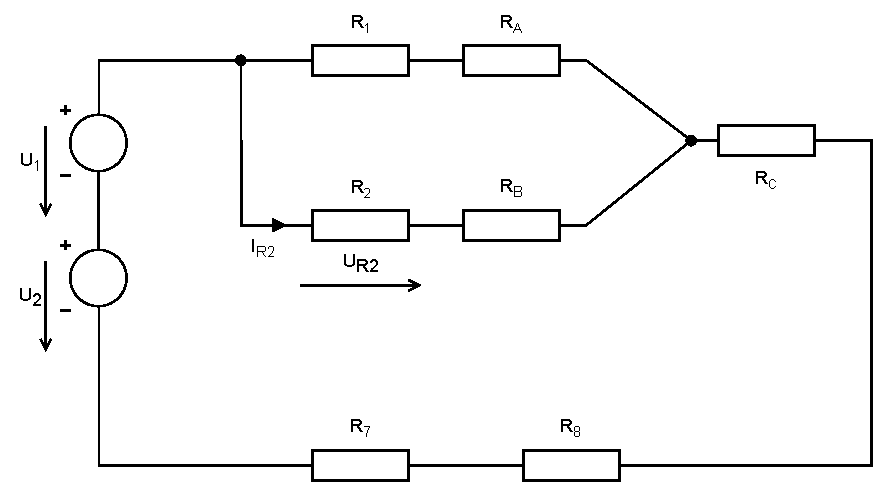
\includegraphics[scale=0.8,keepaspectratio]{fig/solutions/01-sol/01-step2.pdf} \\
Obr.1.2 - Transfigurace - Trojuhelník $\Rightarrow$ Hvězda
\end{center}


\begin{gather*}
% R_A
R_A = \frac{R_3 \times R_{56}}{R_3 + R_4 + R_{56}} =
\frac{410 \times 243.24324324}{410 + 130 + 243.24324324}=
127.32919255\Omega \\\\
% R_B
R_B = \frac{R_3 \times R_4}{R_3 + R_4 + R_{56}} =
\frac{410 \times 130}{410 + 130 + 243.24324324} =
68.05037957 \Omega \\\\
% R_C
R_C = \frac{R_4 \times R_{56}}{R_3 + R_4 + R_{56}} =
\frac{130 \times 243,2432}{410 + 130 + 243.24324324} =
40.37267081 \Omega
\end{gather*}

%%% Krok 3 - Zjednodušení sériových rezistorů
\begin{center}
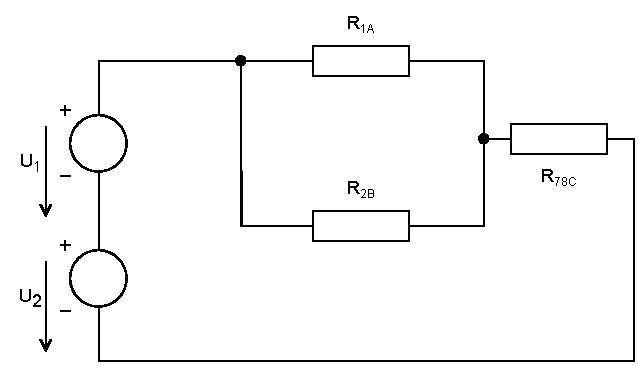
\includegraphics[scale=0.8,keepaspectratio]{fig/solutions/01-sol/01-step3.pdf} \\
Obr.1.3 - Zjednodušení sériových rezistorů \\
($R_7, R_8, R_C, \Rightarrow R_{78C}$ | $R_1, R_A \Rightarrow R_{1A}$ | $R_2, R_B \Rightarrow R_{2B}$)
\end{center}

\begin{gather*}
%R_78C
R_{78C} = R_7 + R_8 + R_C =
310 + 190 + 40.37267081 =
540.37267081 \Omega
\\\\
% R_1A
R_{1A} = R_1 + R_A =
350 + 127.32919255 =
477.32919255 \Omega
\\\\
% R_{2B}
R_{2B} = R_2 + R_B =
650 + 68.05037957 =
718.05037957 \Omega
\end{gather*}

\newpage

%%% Krok 4 - Zjednodušení paralelných rezistorů
\begin{center}
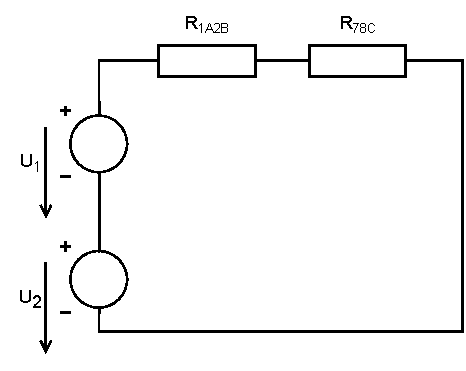
\includegraphics[scale=0.8,keepaspectratio]{fig/solutions/01-sol/01-step4.pdf} \\
Obr.1.4 - Zjednodušení paralelných rezistorů
($R_{1A}, R_{2B} \Rightarrow R_{1A2B}$)
\end{center}

\begin{gather*}
    % R_1A2B
    R_{1A2B} = \frac{R_{1A} \times R_{2B}}{R_{1A} + R_{2B}} =
    \frac{477.32919255 \times 718.05037957}{477.32919255 + 718.05037957} =
    286.72600393 \Omega
\end{gather*}

%%% Krok 5 - Zjednodušení sériových rezistorů a napětí
\begin{center}
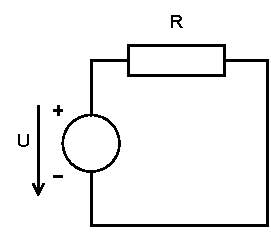
\includegraphics[scale=0.8,keepaspectratio]{fig/solutions/01-sol/01-step5.pdf} \\
Obr.1.5 - Zjednodušení sériových rezistorů
($R_{1A2B}, R_{78C} \Rightarrow R$)
\end{center}

\begin{gather*}
    % R
    R = R_{1A2B} + R_{78C} = 286.72600393 + 540.37267081 = 827.09867473 \Omega \\
\end{gather*}

Zjednodušení napětí
($U_1, U_2 \Rightarrow U$)
\begin{gather*}
    % U
    U = U_1 + U_2 = 80 + 120 = 200 V \
\end{gather*}

Výpočet proudu
\begin{gather*}
    % I
    I = \frac{U}{R} = \frac{200}{827.09867473} = 0.24180912 A \\
\end{gather*}

\newpage

\noindent Teď můžeme provést zpětný výpočet pomocí kroků 4 a 3 $\boldsymbol{U_{R_2}}$ a $\boldsymbol{I_{R_2}}$:
\\\\
Vypočítejme úbytek napětí na $R_{1A2B}$ pomocí proudu, který se v sériovém obvodu nemění.

\begin{gather*}
    % U_R1A2b
    U_{R_{1A2B}} = I \times R_{1A2B} = 0.2418 \times 286.72600393 = 69.33296176 V \\\\
    U_{R_{2B}} = U_{R_{1A2B}} \\
\end{gather*}

\noindent Protože víme, že úbytek napětí je v paralelním obvodu stejný, můžeme vypočítat proud, který prochází dolní větví.

\begin{gather*}
    % I_R2
    \boldsymbol{I_{R_2}} = I_{R_{2B}} = \frac{U_{R_{2B}}}{R_{2B}} =
    \frac{69.33296176}{718.05037957} =
    \textbf{0.09655724A} \\\\
\end{gather*}

\noindent Dopočítame úbytok napätia na $\boldsymbol{U_{R_2}}$:

\begin{gather*}
    \boldsymbol{U_{R_2}} = I_{R_2} \times R_2 = 0.09655724 \times 650 = \textbf{62.76220503V}
\end{gather*}

